\xchapter{Evaluation}{}\label{chap:evaluation}

In this chapter, we evaluate our model by solving two variations of the source code attribution problem. In Section \ref{sec:validation}, we describe how we selected the parameters of our model. In Section \ref{sec:matching}, we solve the authorship matching problem suggested in Chapter \ref{chap:methodology}. In Section \ref{sec:one_to_many}, we solve a closed-world identification problem.

\section{Training and Selection}\label{sec:validation}

We trained and validated the proposed model with Tensorflow. We picked the training samples from a balanced dataset with 20,000 C++ examples from 1,000 authors. A validation set was built from another 3,200 samples from 400 authors. No author from the training set was present on the validation set. All the samples were extracted from the Codeforces dataset.

Although programming competitions resemble laboratory conditions, it is common for participants to code on top of a pre-written file, usually called \textit{template}. Although the constructions present on a template file are usually written by the author himself, they are not always used by the piece of code actually written during the competition. Therefore, it is interesting to analyze how classifiers perform when such constructions are stripped out of the code. For that end, we used \textit{clang}\footnote{\url{https://clang.llvm.org}} to remove unused pieces of code from a C++ program. Moreover, we also removed macros, a construction heavily present in templates of competitive programmers. Therefore, we built two versions of each dataset: one composed of raw source codes and other composed of codes processed by \textit{clang}.

We optimized the model parameters with \textit{RMSprop} \cite{rmsprop} for a maximum of 50 epochs, or until the evaluated equal error rate (EER) of the model on the validation set had no improvement for 5 epochs. We used a learning rate of $10^{-3}$. The version that yielded the highest EER was taken as the final model. During this process, we carefully tuned its hyperparameters.

Finally, we trained two different models with such hyperparameters: one on the raw version of the dataset and other on the \textit{clang} processed version.

\section{Matching Two Unknown Source Codes}\label{sec:matching}

\begin{figure}[ht]
	\centering
	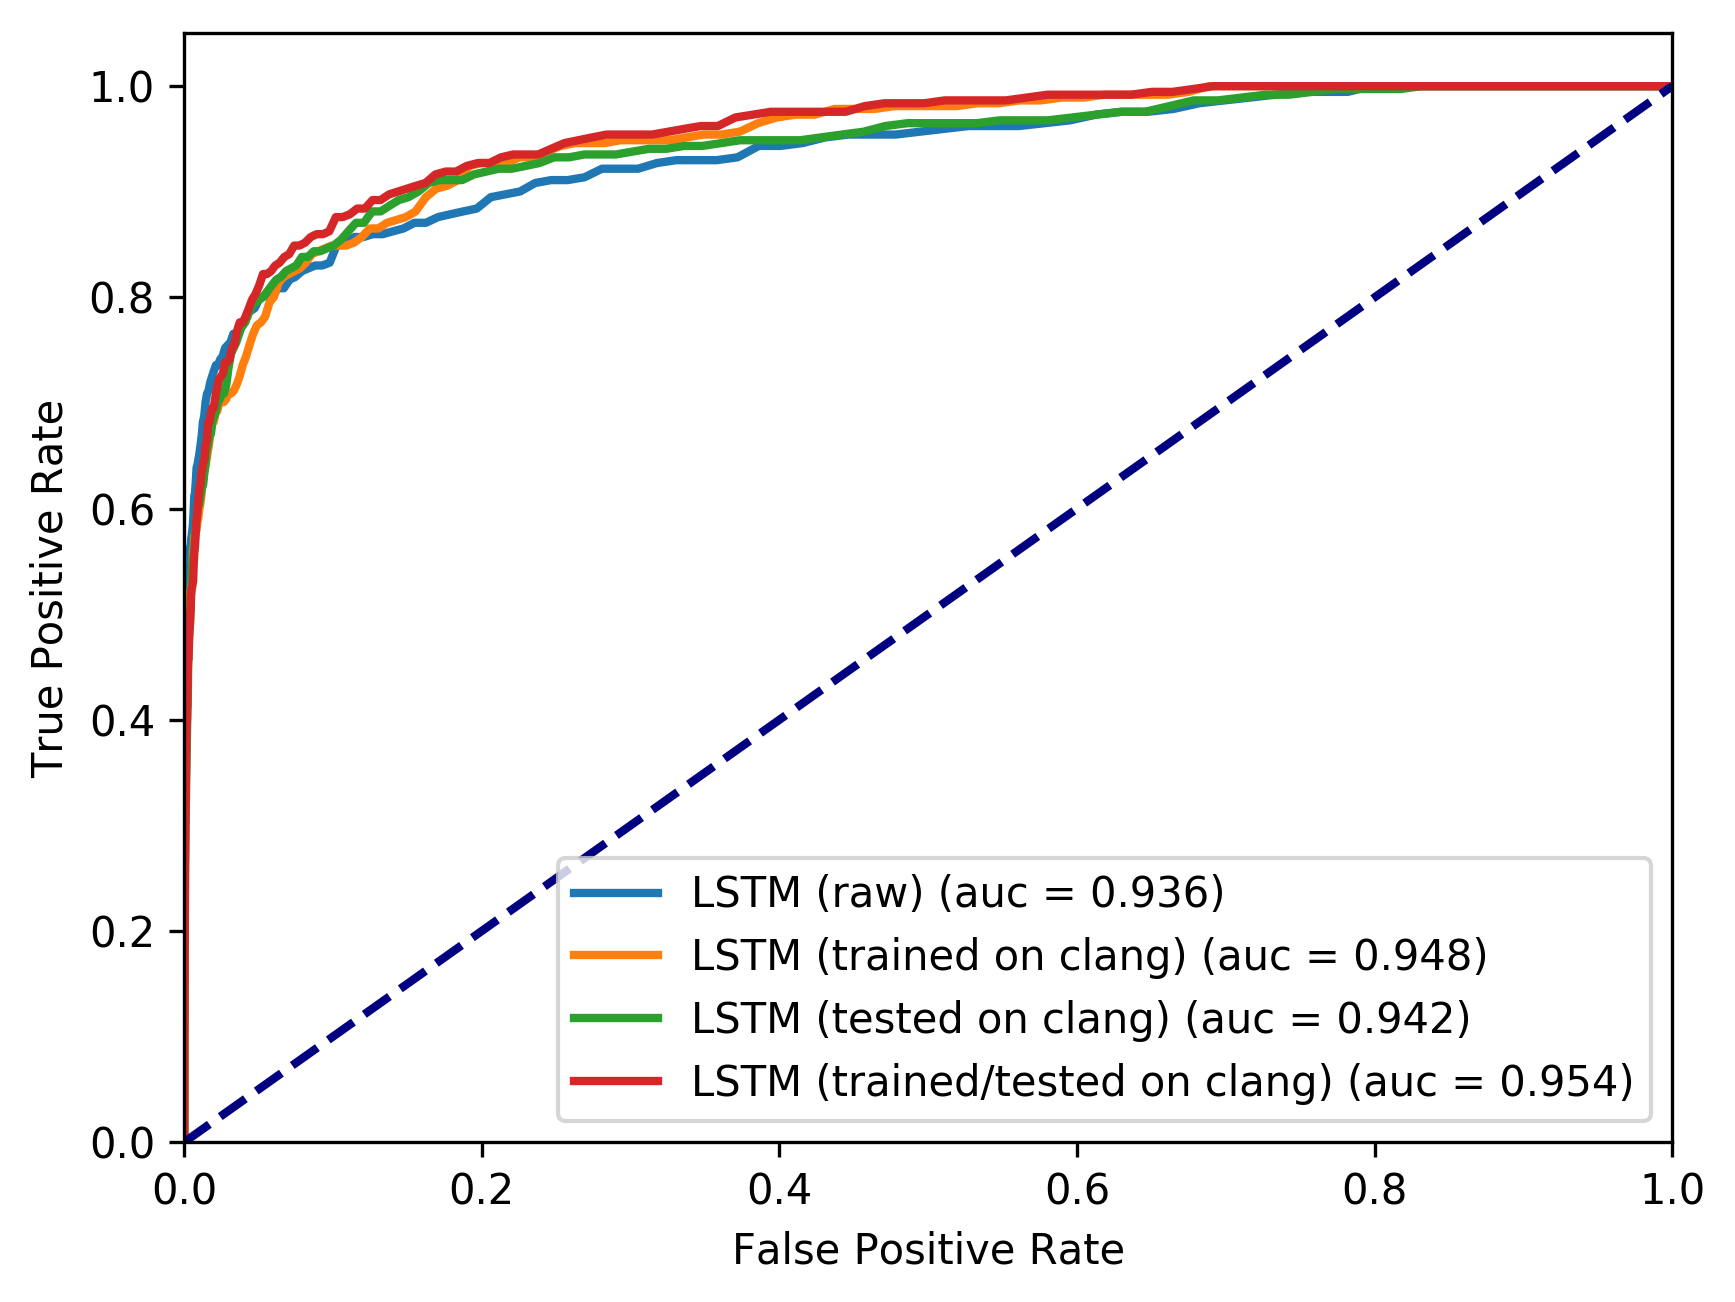
\includegraphics[width=0.7\linewidth]{imgs/roc_complete.png}
	\caption{ROC curve for each pair of classifier and dataset version.}
	\label{fig:roc_complete}
\end{figure}

Using the models we trained, we tried to solve the problem of deciding if two source codes are from the same author. For that end, we constructed a test dataset with 3,200 samples from 400 authors. These samples were extracted from the Codeforces dataset, but this set has no intersection of authors with the training and validation sets used to train the models. Therefore, the authors are unknown to the system. Moreover, we ran \textit{clang} on the samples, obtaining a \textit{clang} processed version of the test dataset.

Finally, we ran four evaluations, one for each combination of model and test dataset. The results can be seen in Fig. \ref{fig:roc_complete} and  Table \ref{tab:matching}.

\begin{table}[ht]
	\centering
	\begin{tabular}{ccr}
		\cline{2-3}
		\multicolumn{1}{l}{}                     & \multicolumn{2}{c}{\textbf{EER (\%)}}                                   \\ \cline{2-3} 
		\textbf{}                                & \textbf{Raw Test Set}     & \multicolumn{1}{l}{\textbf{\textit{clang} Test Set}} \\ \hline
		
		%\textbf{CNN (trained on raw version)}   & \multicolumn{1}{r}{16.31} & 16.88                                       \\ \hline
		%\textbf{CNN (trained on \textit{clang} version)} & \multicolumn{1}{r}{16.82} & 16.90                                        \\ \hline
		
		\textbf{LSTM (trained on raw version)}   & \multicolumn{1}{r}{13.88} & 12.24                                       \\ \hline
		\textbf{LSTM (trained on \textit{clang} version)} & \multicolumn{1}{r}{13.25} & 11.60                                        \\ \hline
	\end{tabular}
	\caption{Equal error rate (EER) evaluation of the trained models on each test set.}
	\label{tab:matching}
\end{table}

We can notice that the performance on raw source codes is slightly worse than the others. This can be related to the fact that tested authors are not present in training and validation sets. The model is probably relying more on features present on templates, instead of on stylistic features of the written code. Therefore, the embeddings generalize poorly to unknown authors. The better performance of the \textit{clang} combination supports this claim by showing that learning from features of the written code yields better generalization.

\section{One-to-Many Author Identification}\label{sec:one_to_many}

We also evaluated our models on the problem posed by \citeauthoronline{caliskan_2015}. In their work, 9 C++ source codes from 250 programmers are extracted from the Google Code Jam dataset. From these, 8 are used for training and one for testing. We simply took the models we trained for the previous experiment , added a fully-connected layer and replaced triplet loss with softmax cross-entropy loss. Then, we trained this layer on the $250 \times 8$ source codes for more epochs.

The rank-$n$ metric evaluations, for $n = 1$ and $n = 3$, can be seen in Table \ref{tab:rank}.

\begin{table}[hb]
	\centering
	\begin{tabular}{lrrrr}
		\cline{2-5}
		& \multicolumn{2}{c}{\textbf{rank-1 (\%)}}                                        & \multicolumn{2}{c}{\textbf{rank-3 (\%)}}                                        \\ \cline{2-5} 
		\multicolumn{1}{c}{\textbf{}}    & \multicolumn{1}{c}{\textbf{Raw Test}} & \multicolumn{1}{l}{\textbf{Clang Test}} & \multicolumn{1}{l}{\textbf{Raw Test}} & \multicolumn{1}{l}{\textbf{Clang Test}} \\ \hline
		\textbf{LSTM (trained on raw)}   & 74.8\%                                & 67.0\%                                    & 84.4\%                                & 79.6\%                                  \\ \hline
		\textbf{LSTM (trained on clang)} & 65.0\%                                  & 69.0\%                                    & 78.8\%                                & 82.8\%                                  \\ \hline
		\textbf{\citeauthoronline{caliskan_2015}}                & 95.1\%                               & n/a                                     & n/a                                   & n/a                                     \\ \hline
	\end{tabular}
	\caption{Rank-$n$ metric for the one-to-many identification problem on 250 programmers of the Google Code Jam dataset. }
	\label{tab:rank}
\end{table}

Although we were not able to match the Random Forest model proposed by \citeauthoronline{caliskan_2015}, we are able to show that the generated descriptors are discriminative. Fig. \ref{fig:embedding} shows the style descriptors of source codes from 12 programmers of Google Code Jam dataset. They were embedded into a two-dimensional space for better visualization.

\begin{figure}[ht]
	\centering
	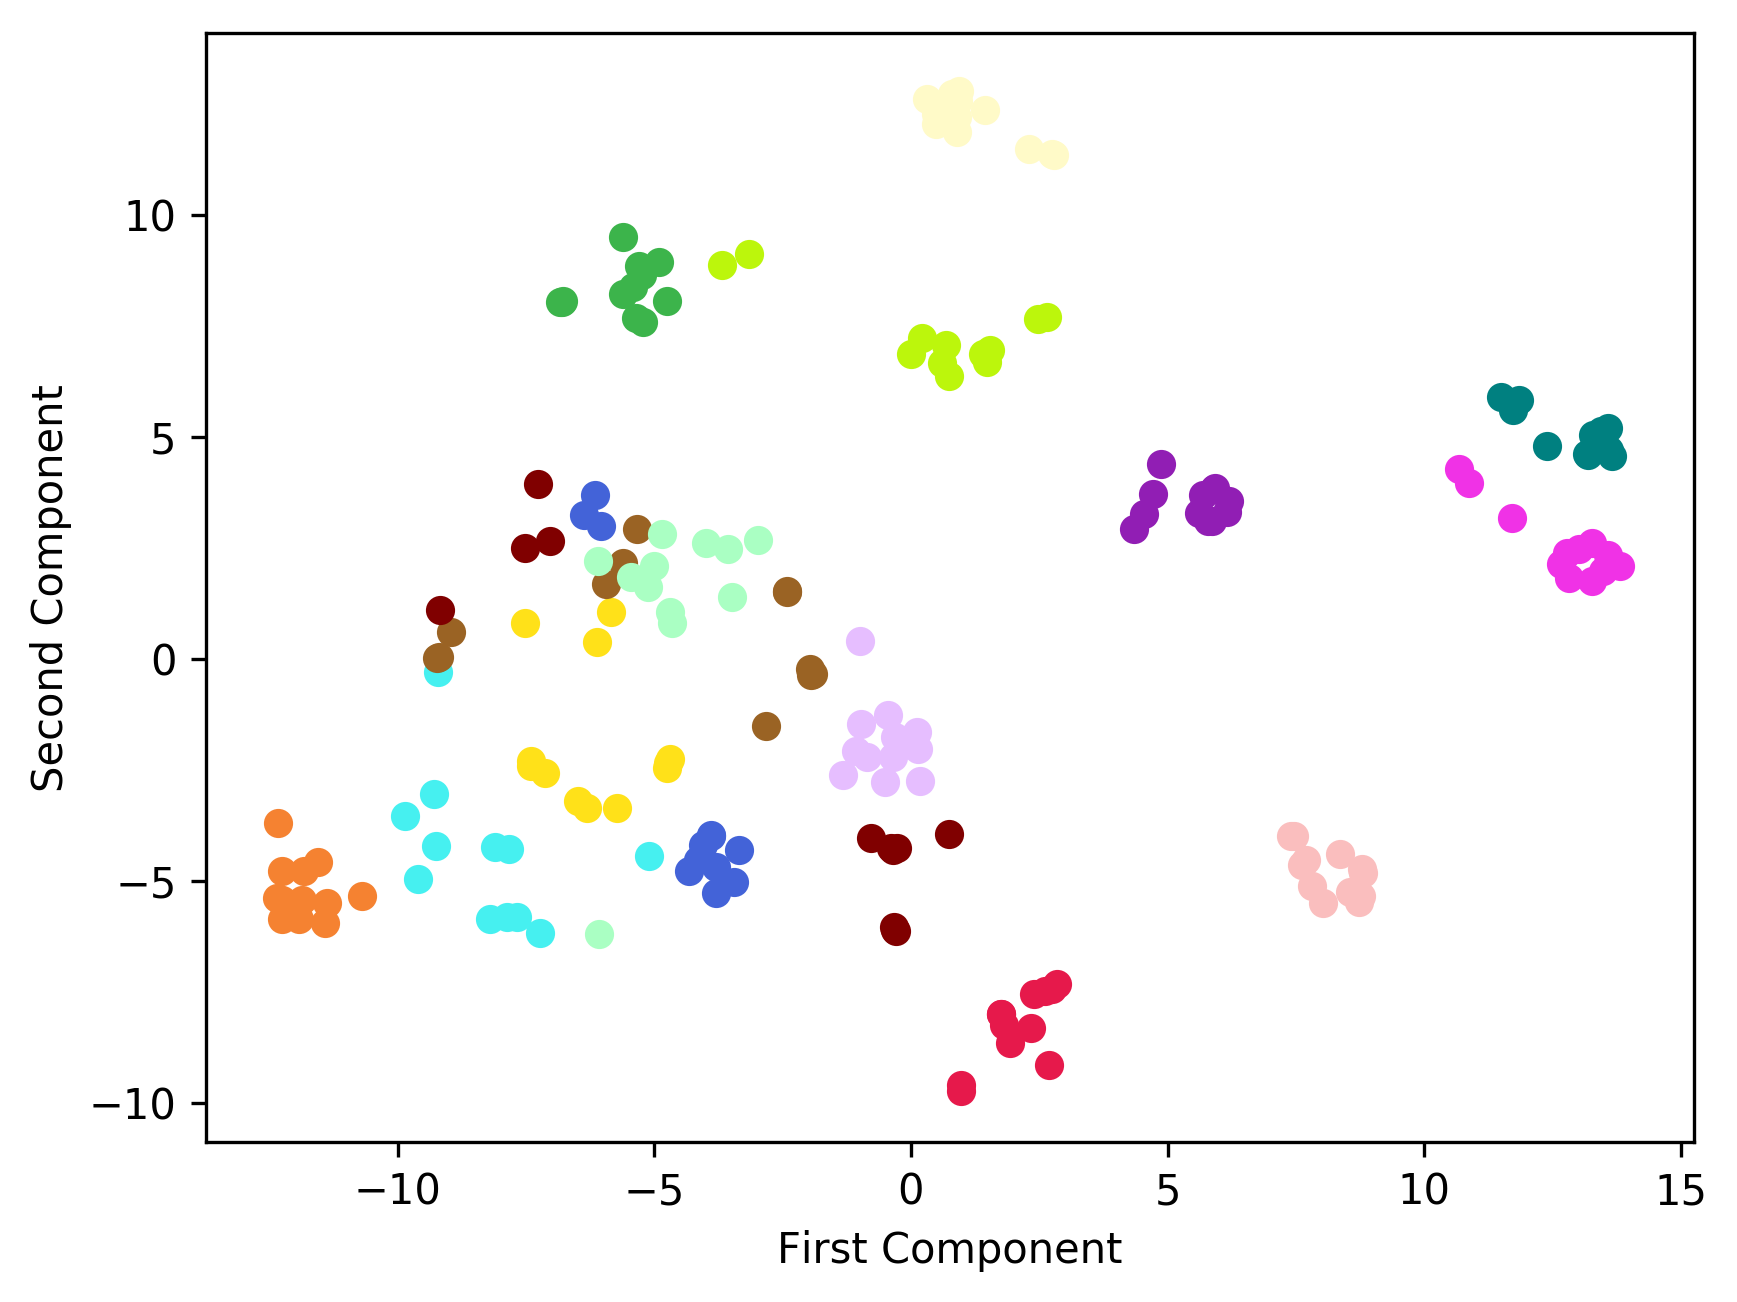
\includegraphics[width=0.7\linewidth]{imgs/embedding.png}
	\caption{128-dimensional descriptors from 12 authors generated by the LSTM model, trained and test on the \textit{clang} test set. The descriptors were embedded into a two-dimensional space with t-SNE.}
	\label{fig:embedding}
\end{figure}